\section{Analysis of vegetation density}
\label{sec:vegetation_analysis}
After the segmentation of the surface into different classes, the second objective of this thesis is to draw conclusions on vegetation density. Vegetation is one of the main factors to consider when looking for suitable emergency landing fields. Lower vegetation density increases the chances of a successful emergency landing.

One method for analyzing vegetation density with remotely sensed data are \emph{spectral vegetation indices}. This chapter focuses on investigating several spectral vegetation indices and their usefulness with the data set presented in chapter~\ref{sec:dataset_analysis}.

\subsection{Spectral Vegetation Indices}
Spectral vegetation indices provide ways to indicate the vegetation density based on reflectances of visible and near-infrared (NIR) light spectrums. They rely on the fact that healthy vegetation absorbs most of the visible red and blue light while reflecting great portions of green light~\cite{glv03}.

Actually, the reflections of green light on plants is significantly higher than all other spectrums. This is what makes plants and vegetation appear green to the human eye. Other materials on earth's surface do not share this increased reflectance levels in the green spectrum. Building upon this knowledge, SVIs try to relate different spectral bands of light to predict vegetation density.

Most SVIs compare the difference between visible red light and NIR light~\cite{glv03}. The lower the amount of red light, the higher the density of green vegetation in the scene.

There are various indices that each combine the spectral bands in unique ways and perform slightly different color corrections. Most of the indices use simple algebraic formulas. In the end, they all produce a single scalar value indicating the density of the vegetation.

The next sections introduce some of the widely used vegetation indices.

\subsubsection{Ratio Vegetation Index}
The simplest SVI is the \emph{Ratio Vegetation Index} (RVI). It is represented by the ratio between NIR and red light~\cite{glv03} (see equation~\ref{eq:rvi}). Higher values indicate denser vegetation.

\begin{equation}
    \text{RVI} = \frac{\text{NIR}}{\text{Red}}
    \label{eq:rvi}
\end{equation}

Non-vegetated areas typically are below or near $1$. In that case the reflectance for NIR and red light are in the same order of magnitude. With increasing vegetation density, the amount of reflected red light shrinks, causing the index to grow. Extremely dense vegetation reaches a size of up to $30$.

The lower bound for the index is $0$, because negative values for the reflectances are not possible. On the other hand, there is no upper limit for the index. This makes it difficult to define from when exactly a vegetation is considered to be dense.

\subsubsection{Normalized Difference Vegetation Index}
One of the first approaches to monitor changes in global vegetation was driven by the National Oceanic and Atmospheric Administration (NOAA), a US agency focusing on the conditions of the environment. With the help of satellites and high-resolution radiometers they measured the earth's reflectance in five spectral bands, including red and NIR wavelengths. To support their analysis, they introduced a new vegetation index called the \emph{Normalized Difference Vegetation Index} (NDVI)~\cite{measuring_vegetation00}.

The NDVI was able to solve some of the shortcomings of the RVI. For example, because of the way it is calculated (see equation~\ref{eq:ndvi}), it is limited to the range of $-1$ to $1$. This makes it easier to categorize density levels for vegetation.

\begin{equation}
    \text{NDVI} = \frac{\text{NIR}-\text{Red}}{\text{NIR}+\text{Red}}
    \label{eq:ndvi}
\end{equation}

Values close to $1$ indicate a high probability for dense, green vegetation~\cite{gisg_ndvi20}. For lower values the density of the vegetation decreases. Values near $0$ do not allow for any precise conclusions about the surface conditions, except that living vegetation is very unlikely at that location. The negative range of values mostly consists of water.

\subsubsection{Enhanced Vegetation Index}
As time passes, improved measuring instruments were launched, like the Terra mission\footnote{see \url{https://terra.nasa.gov/}} of the National Aeronautics and Space Administration (NASA). The new instruments not only increased the resolution but also the precision of the spectral analysis. The more accurate data led to adjustments in the calculations for vegetation density, eventually resulting in the \emph{Enhanced Vegetation Index} (EVI)~\cite{modis2002}.

The EVI is calculated similarly to the NDVI, but has some additional factors to correct the influence of atmospheric conditions and background noise (see equation~\ref{eq:evi}). This means that EVI is more sensitive and offers more reliable information about the vegetation.

\begin{equation}
    \text{EVI} = G * \frac{
    \text{NIR}-\text{Red}
    }{
    \text{NIR} + C_1 * \text{Red} - C_2 * \text{Blue} + L
    }
    \label{eq:evi}
\end{equation}

$C_1$ and $C_2$ are coefficients to reduce the effects of aerosols. To filter out the distortions in the best possible way, also the spectral band of blue light is consulted for this. $L$ is a constant adjustment to address the issues of canopy background noise. Finally, $G$ is called the \emph{gain factor} and is used for linear scaling of the index. The values chosen in the original Terra mission are $C_1=6$, $C_2=7.5$, $L=1$ and $G=2.5$~\cite{modis2002}.

\subsubsection{Soil-Adjusted Vegetation Indices}
\WIP{
another approach to improve NDVI is \emph{Soil Adjusted Vegetation Index} (SAVI) \cite{savi88}. Huete found NDVI to be unstable with factors like soil color and moisture. Introduced a canopy background adjustment factor $L$ to correct unwanted influence of soil variations. In his experiments, he found value of $L=0.5$ works best to eliminate side effects without further calibration. equation \ref{eq:savi} shows exact calculation.

\begin{equation}
    \displaystyle
    \text{SAVI} =
    \bigg(
    \frac{\text{NIR} - \text{Red}}
    {\text{NIR} + \text{Red} + L}
    \bigg) * \big(1 + L \big)
    \label{eq:savi}
\end{equation}

one issue with SAVI is that proper soil adjustment depends on vegetation density. Without prior knowledge regarding vegetation it is hard to find value of $L$ that works good for everything. Qi et~al. presented a functional $L$ factor to replace in SAVI. Calculation shown in \ref{eq:msavi}. entire derivation is to be found in \cite{msavi94}.

\begin{equation}
    \displaystyle
    \text{MSAVI} = \frac
    {
    2 \text{NIR} + 1
    - \sqrt{
    \big(2 \text{NIR}\big)^2
    - 8 \big(\text{NIR} - \text{Red}\big)
    }
    }
    {2}
    \label{eq:msavi}
\end{equation}
}

\subsection{Experiments}
\WIP{
\begin{itemize}
    \item compute vegetation indices for some images
    \item compare results to the real landscape in the dataset
\end{itemize}
}

\newcommand{\VegetationIndicesImageWidth}{0.18\textwidth}
% INFO: no upper bound for RVI. Calculated biggest values and interpolated from 0-20 to 0-255 for visualization
\begin{figure}
    \centering

    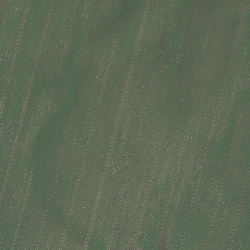
\includegraphics[width=\VegetationIndicesImageWidth]{images/vegetation/original/1} \hfill
    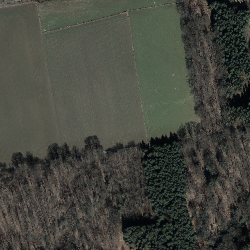
\includegraphics[width=\VegetationIndicesImageWidth]{images/vegetation/original/2} \hfill
    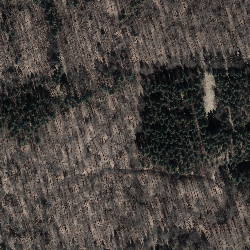
\includegraphics[width=\VegetationIndicesImageWidth]{images/vegetation/original/3} \hfill
    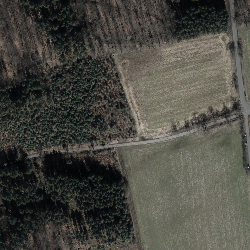
\includegraphics[width=\VegetationIndicesImageWidth]{images/vegetation/original/4} \hfill
    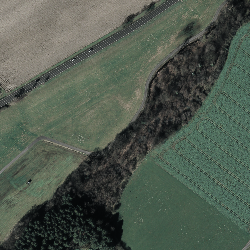
\includegraphics[width=\VegetationIndicesImageWidth]{images/vegetation/original/5}

    \vspace{3mm}
    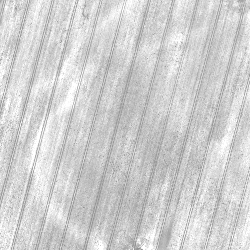
\includegraphics[width=\VegetationIndicesImageWidth]{images/vegetation/rvi/1} \hfill
    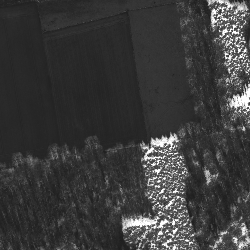
\includegraphics[width=\VegetationIndicesImageWidth]{images/vegetation/rvi/2} \hfill
    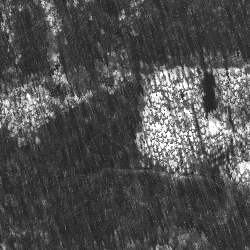
\includegraphics[width=\VegetationIndicesImageWidth]{images/vegetation/rvi/3} \hfill
    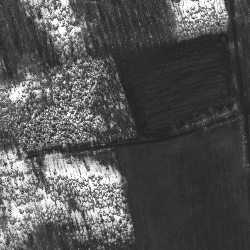
\includegraphics[width=\VegetationIndicesImageWidth]{images/vegetation/rvi/4} \hfill
    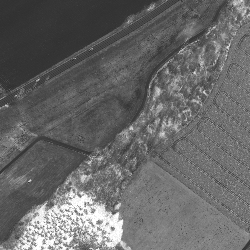
\includegraphics[width=\VegetationIndicesImageWidth]{images/vegetation/rvi/5}

    \caption{Vegetation analysis using RVI}
    \label{fig:vegetation_rvi_examples}
\end{figure}

\begin{figure}
    \centering

    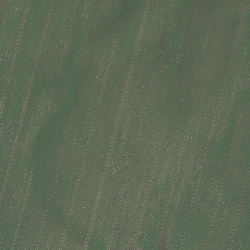
\includegraphics[width=\VegetationIndicesImageWidth]{images/vegetation/original/1} \hfill
    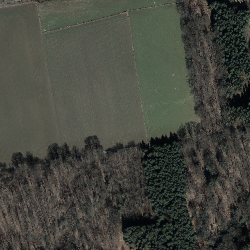
\includegraphics[width=\VegetationIndicesImageWidth]{images/vegetation/original/2} \hfill
    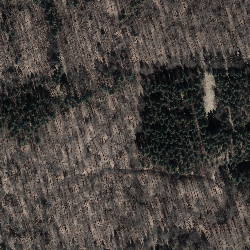
\includegraphics[width=\VegetationIndicesImageWidth]{images/vegetation/original/3} \hfill
    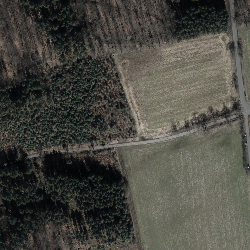
\includegraphics[width=\VegetationIndicesImageWidth]{images/vegetation/original/4} \hfill
    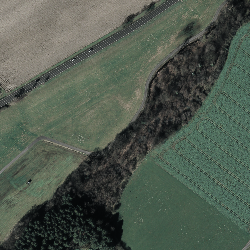
\includegraphics[width=\VegetationIndicesImageWidth]{images/vegetation/original/5}

    \vspace{3mm}
    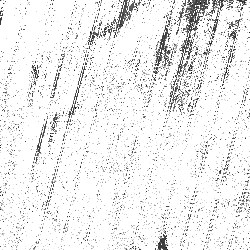
\includegraphics[width=\VegetationIndicesImageWidth]{images/vegetation/ndvi/1} \hfill
    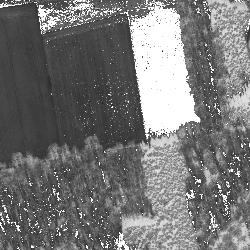
\includegraphics[width=\VegetationIndicesImageWidth]{images/vegetation/ndvi/2} \hfill
    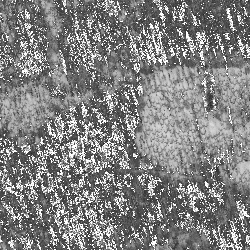
\includegraphics[width=\VegetationIndicesImageWidth]{images/vegetation/ndvi/3} \hfill
    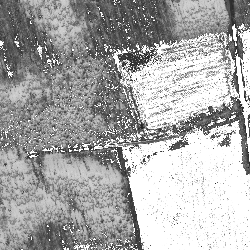
\includegraphics[width=\VegetationIndicesImageWidth]{images/vegetation/ndvi/4} \hfill
    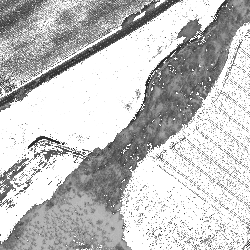
\includegraphics[width=\VegetationIndicesImageWidth]{images/vegetation/ndvi/5}

    \caption{Vegetation analysis using NDVI}
    \label{fig:vegetation_ndvi_examples}
\end{figure}

\begin{figure}
    \centering

    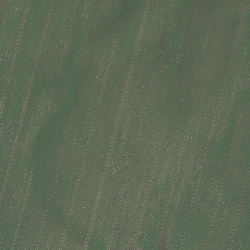
\includegraphics[width=\VegetationIndicesImageWidth]{images/vegetation/original/1} \hfill
    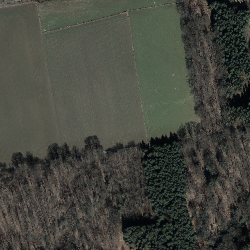
\includegraphics[width=\VegetationIndicesImageWidth]{images/vegetation/original/2} \hfill
    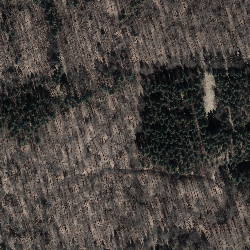
\includegraphics[width=\VegetationIndicesImageWidth]{images/vegetation/original/3} \hfill
    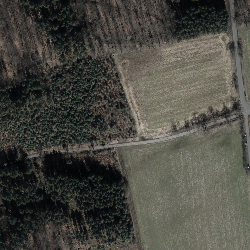
\includegraphics[width=\VegetationIndicesImageWidth]{images/vegetation/original/4} \hfill
    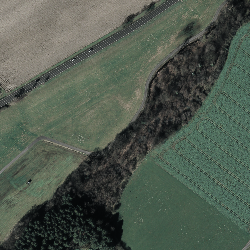
\includegraphics[width=\VegetationIndicesImageWidth]{images/vegetation/original/5}

    \vspace{3mm}
    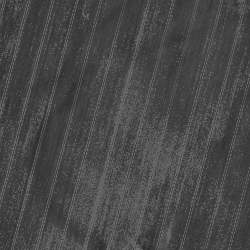
\includegraphics[width=\VegetationIndicesImageWidth]{images/vegetation/evi/1} \hfill
    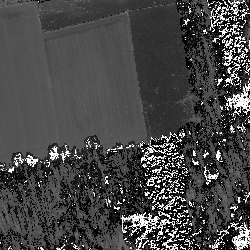
\includegraphics[width=\VegetationIndicesImageWidth]{images/vegetation/evi/2} \hfill
    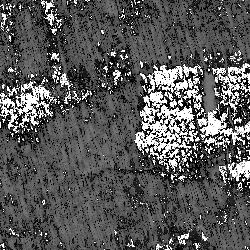
\includegraphics[width=\VegetationIndicesImageWidth]{images/vegetation/evi/3} \hfill
    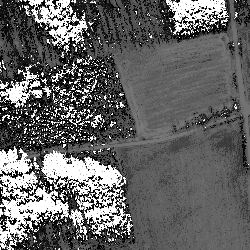
\includegraphics[width=\VegetationIndicesImageWidth]{images/vegetation/evi/4} \hfill
    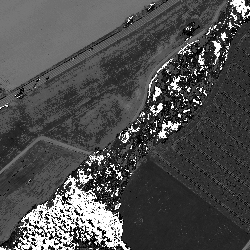
\includegraphics[width=\VegetationIndicesImageWidth]{images/vegetation/evi/5}

    \caption{Vegetation analysis using EVI}
    \label{fig:vegetation_evi_examples}
\end{figure}

% INFO: no bounds for (M)SAVI. Interpolated from SAVI 0-20, MSAVI 0-80
\begin{figure}
    \centering

    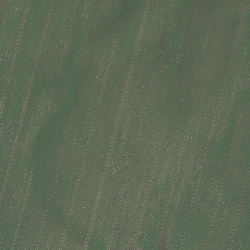
\includegraphics[width=\VegetationIndicesImageWidth]{images/vegetation/original/1} \hfill
    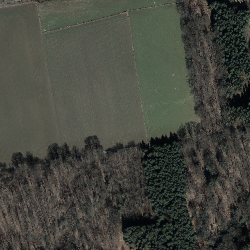
\includegraphics[width=\VegetationIndicesImageWidth]{images/vegetation/original/2} \hfill
    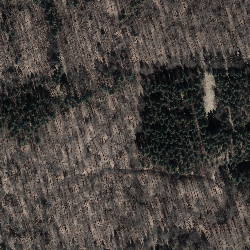
\includegraphics[width=\VegetationIndicesImageWidth]{images/vegetation/original/3} \hfill
    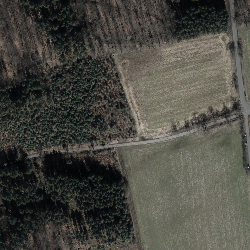
\includegraphics[width=\VegetationIndicesImageWidth]{images/vegetation/original/4} \hfill
    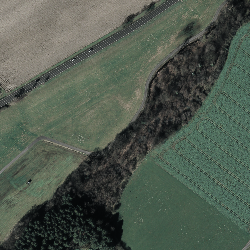
\includegraphics[width=\VegetationIndicesImageWidth]{images/vegetation/original/5}

    \vspace{3mm}
    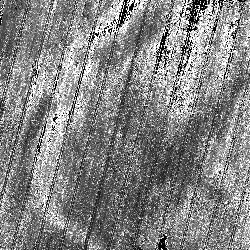
\includegraphics[width=\VegetationIndicesImageWidth]{images/vegetation/savi/1} \hfill
    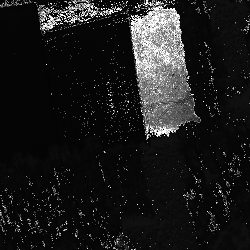
\includegraphics[width=\VegetationIndicesImageWidth]{images/vegetation/savi/2} \hfill
    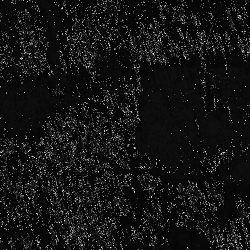
\includegraphics[width=\VegetationIndicesImageWidth]{images/vegetation/savi/3} \hfill
    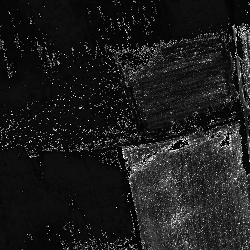
\includegraphics[width=\VegetationIndicesImageWidth]{images/vegetation/savi/4} \hfill
    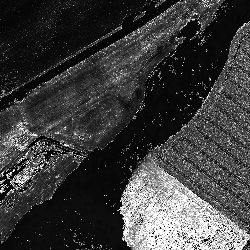
\includegraphics[width=\VegetationIndicesImageWidth]{images/vegetation/savi/5}

    \vspace{3mm}
    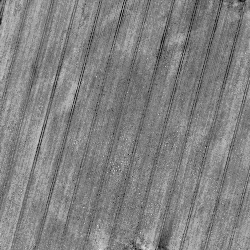
\includegraphics[width=\VegetationIndicesImageWidth]{images/vegetation/msavi/1} \hfill
    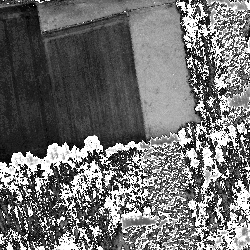
\includegraphics[width=\VegetationIndicesImageWidth]{images/vegetation/msavi/2} \hfill
    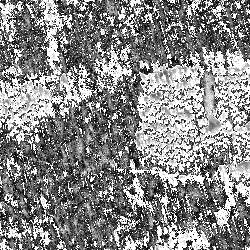
\includegraphics[width=\VegetationIndicesImageWidth]{images/vegetation/msavi/3} \hfill
    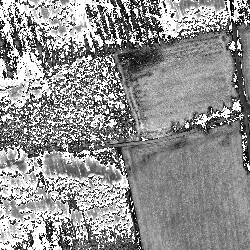
\includegraphics[width=\VegetationIndicesImageWidth]{images/vegetation/msavi/4} \hfill
    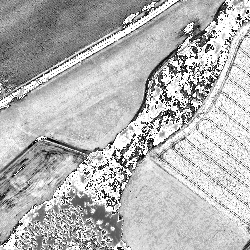
\includegraphics[width=\VegetationIndicesImageWidth]{images/vegetation/msavi/5}

    \caption{Vegetation analysis using SAVI and MSAVI}
    \label{fig:vegetation_savi_examples}
\end{figure}

\subsection{Discussion}
\WIP{
\begin{itemize}
    \item raise concerns about dataset limitation regarding the indices
    \item discuss practical use of those results for identifying emergency landing fields
\end{itemize}
}

\newpage
